% !TeX spellcheck = en_GB
%%%%%%%%%%%%%%%%%%%%%%%%%%%%%%%%%%%%%%%%%%
%                                        %
%    Engineer thesis LaTeX template      % 
%                                        %
%%%%%%%%%%%%%%%%%%%%%%%%%%%%%%%%%%%%%%%%%%
%  (c) Krzysztof Simiński, 2018-2022     %
%%%%%%%%%%%%%%%%%%%%%%%%%%%%%%%%%%%%%%%%%%

% compilation:

% pdflatex thesis
% biber    thesis
% pdflatex thesis
% pdflatex thesis 

%%%%%%%%%%%%%%%%%%%%%%%%%%%%%%%%%%%%%%%%%%

\documentclass[a4paper,twoside,12pt]{book}
\usepackage[utf8]{inputenc}                                      
\usepackage[T1]{fontenc}
\usepackage{amsmath,amsfonts,amssymb,amsthm}
\usepackage[polish,british]{babel} 
\usepackage{indentfirst}
\usepackage{lmodern}
\usepackage{graphicx} 
\usepackage{hyperref}
\usepackage{booktabs}
%\usepackage{tikz}
%\usepackage{pgfplots}
\usepackage{mathtools}
\usepackage{geometry}
\usepackage[page]{appendix} 


%%% My packages %%%
\usepackage{minted}  
\usepackage{algorithm}
\usepackage{algpseudocode}
%%%%%%%%%%%%%%%%%%%%%%%%%%

\usepackage{booktabs}
\usepackage{csquotes}
\usepackage[natbib=true]{biblatex}
\bibliography{bibliography}


\usepackage{setspace}
\onehalfspacing


\frenchspacing

\usepackage{listings}
\lstset{
	language={java},
	basicstyle=\ttfamily,
	keywordstyle=\lst@ifdisplaystyle\color{blue}\fi,
	commentstyle=\color{gray}
}

%%%%%%%%%
 

%%%%%%%%%%%% FANCY HEADERS %%%%%%%%%%%%%%%

\usepackage{fancyhdr}
\pagestyle{fancy}
\fancyhf{}
\fancyhead[LO]{\nouppercase{\it\rightmark}}
\fancyhead[RE]{\nouppercase{\it\leftmark}}
\fancyhead[LE,RO]{\it\thepage}


\fancypagestyle{onlyPageNumbers}{%
   \fancyhf{} 
   \fancyhead[LE,RO]{\it\thepage}
}

\fancypagestyle{PageNumbersChapterTitles}{%
   \fancyhf{} 
   \fancyhead[LO]{\nouppercase{\it\rightmark}}
   \fancyhead[RE]{\nouppercase{\it\leftmark}}
   \fancyhead[LE,RO]{\it\thepage}
}


%%%%%%%%%%%%%%%%%%%%%%%%%%%
% listings 
\usepackage{listings}
\lstset{%
language=C++,%
commentstyle=\textit,%
identifierstyle=\textsf,%
keywordstyle=\sffamily\bfseries, %\texttt, %
%captionpos=b,%
tabsize=3,%
frame=lines,%
numbers=left,%
numberstyle=\tiny,%
numbersep=5pt,%
breaklines=true,%
morekeywords={descriptor_gaussian,descriptor,partition,fcm_possibilistic,dataset,my_exception,exception,std,vector},%
escapeinside={@*}{*@},%
%texcl=true, % wylacza tryb verbatim w komentarzach jednolinijkowych
}
%%%%%%%%%%%%%%%%%%%%%%%%%%%%%%%%%%%%

%%%% TODO LIST GENERATOR %%%%%%%%%

\usepackage{color}
\definecolor{brickred}      {cmyk}{0   , 0.89, 0.94, 0.28}

\makeatletter \newcommand \kslistofremarks{\section*{Remarks} \@starttoc{rks}}
  \newcommand\l@uwagas[2]
    {\par\noindent \textbf{#2:} %\parbox{10cm}
{#1}\par} \makeatother


\newcommand{\ksremark}[1]{%
{%\marginpar{\textdbend}
{\color{brickred}{[#1]}}}%
\addcontentsline{rks}{uwagas}{\protect{#1}}%
}

%%%%%%%%%%%%%% END OF TODO LIST GENERATOR %%%%%%%%%%% 

% some issues...

\newcounter{PagesWithoutNumbers}

\newcommand{\hcancel}[1]{%
    \tikz[baseline=(tocancel.base)]{
        \node[inner sep=0pt,outer sep=0pt] (tocancel) {#1};
        \draw[red] (tocancel.south west) -- (tocancel.north east);
    }%
}%

\newcommand{\MonthName}{%
  \ifcase\the\month
  \or January% 1
  \or February% 2
  \or March% 3
  \or April% 4
  \or May% 5
  \or June% 6
  \or July% 7
  \or August% 8
  \or September% 9
  \or October% 10
  \or November% 11
  \or December% 12
  \fi}


%%%%%%%%%%%%%%%%%%%%%%%%%%%%%%%%%%%%%%%%%%%%%%
% Helvetica font macros for the title page:
\newcommand{\headerfont}{\fontfamily{phv}\fontsize{18}{18}\bfseries\scshape\selectfont}
\newcommand{\titlefont}{\fontfamily{phv}\fontsize{18}{18}\selectfont}
\newcommand{\otherfont}{\fontfamily{phv}\fontsize{14}{14}\selectfont}

%%%%%%%%%%%%%%%%%%%%%%%%%%%%%%%%%%%%%%%%%%%%%%
%%%%%%%%%%%%%%%%%%%%%%%%%%%%%%%%%%%%%%%%%%%%%%
%%%%%%%%%%%%%%%%%%%%%%%%%%%%%%%%%%%%%%%%%%%%%%
%%%%%%%%%%%%%%%%%%%%%%%%%%%%%%%%%%%%%%%%%%%%%%
%%%%%%%%%%%%%%%%%%%%%%%%%%%%%%%%%%%%%%%%%%%%%%
%%%%%%%%%%%%%%%%%%%%%%%%%%%%%%%%%%%%%%%%%%%%%%
%%%%%%%%%%%%%%%%%%%%%%%%%%%%%%%%%%%%%%%%%%%%%%
\algnewcommand{\algorithmicand}{\textbf{ and }}
\algnewcommand{\algorithmicor}{\textbf{ or }}
\algnewcommand{\algorithmiceq}{\textbf{ == }}
\algnewcommand{\OR}{\algorithmicor}
\algnewcommand{\AND}{\algorithmicand}
\algnewcommand{\EQ}{\algorithmiceq}
\algnewcommand{\var}{\texttt}


\newcommand{\Author}{Szymon Pluta}
\newcommand{\Supervisor}{Krzysztof Simiński, DSc PhD}
\newcommand{\Consultant}{Name Surname, PhD}
\newcommand{\Title}{Data anonymisation web platform}
\newcommand{\Polsl}{Silesian University of Technology}
\newcommand{\Faculty}{Faculty of Automatic Control, Electronics and Computer Science}
\newcommand{\Programme}{Programme: Informatics}


\addbibresource{bibliography.bib}




\begin{document}
\kslistofremarks
\cleardoublepage
	
%%%%%%%%%%%%%%%%%%  Title page %%%%%%%%%%%%%%%%%%% 
\pagestyle{empty}
{
	\newgeometry{top=2.5cm,%
	             bottom=2.5cm,%
	             left=3cm,
	             right=2.5cm}
	\sffamily
	\rule{0cm}{0cm}
	
	\begin{center}
	
\includegraphics[width=45mm]{logo_eng.jpg}
	\end{center} 
	\vspace{1cm}
	\begin{center}
	\headerfont \Polsl
	\end{center}
	\begin{center}
	\headerfont \Faculty
	\end{center}
	\vfill
	\begin{center}
   \headerfont \Programme
	\end{center}
	\vfill
	\begin{center}
	\titlefont Final Project
	\end{center}
	\vfill
	
	\begin{center}
	\otherfont \Title\par
	\end{center}
	
	\vfill
	
	\vfill
	 
	\noindent\vbox
	{
		\hbox{\otherfont author: \Author}
		\vspace{12pt}
		\hbox{\otherfont supervisor: \Supervisor}
	%	\vspace{12pt} % only if applicable; otherwise delete the line
	%	\hbox{\otherfont consultant: \Consultant} % only if applicable; otherwise delete the line
	}
	\vfill 
 
   \begin{center}
   \otherfont Gliwice,  \MonthName\ \the\year
   \end{center}	
	\restoregeometry
}
  

\cleardoublepage
 

\rmfamily
\normalfont



%%%%%%%%%%%%%%%%%% Table of contents %%%%%%%%%%%%%%%%%%%%%%
\pagenumbering{Roman}
\pagestyle{onlyPageNumbers}
\tableofcontents

%%%%%%%%%%%%%%%%%%%%%%%%%%%%%%%%%%%%%%%%%%%%%%%%%%%%%
\setcounter{PagesWithoutNumbers}{\value{page}}
\mainmatter
\pagestyle{empty}

\chapter*{Abstract}
\addcontentsline{toc}{chapter}{Abstract}

The text of the abstract should be copied into a respective field in the APD system. The Abstract with keywords should not exceed one page.

\paragraph{Keywords:} 2-5 keywords, separated by commas



\cleardoublepage


\pagestyle{PageNumbersChapterTitles}

%%%%%%%%%%%%%% body of the thesis %%%%%%%%%%%%%%%%%


\chapter{Introduction}

Technological advancement being observed in the past years fundamentally changed the relevance of data in today's digitalized world. Information became an innovation stimulus in the area of research and development. The quantity of data that organizations produce, process, store and share is at a continuous growth. An enormous amount of 1.8 zettabytes ($1.8 \cdot 10^{21}$ bytes) of new data was produced only in the 2011, and every two consecutive years this number is doubling \cite{bib:big_data_security}. After decades of observed technological advancement and innovation, the global internet traffic finally entered the zettabyte-era, as it had reached a magnitude of one zettabyte in 2016, and in the calender month being as early as September \cite{bib:cisco_blog}.

The vast quantities of processed information allowed for brand new research fields such as data science or big data analytics to form, which are used by organizations to derive new insights in a way that was previously impossible. Organizations collect and process the data to enhance the services they provide to the customers through statistical analysis or newly developed computer science processes including data mining and machine learning. The utility of delivered services is increased at a lower cost and improved efficiency through the insights extracted from the collected information about how the services are consumed \cite{bib:anonymization_pipeline}.


\vfill

\footnotesize
\color{blue}
Następne do zrobienia, w uproszczeniu i w podanej kolejności:
\begin{itemize}
\item Jak widać, dane są używane wszędzie. Przeciętna osoba sobie nawet nie zdaje sprawy.
\item Istota prywatności danych, ochrona danych osobowych.
\item Prawo wolno reaguje na uregulowanie ochrony danych osobowych: GDPR dopiero w 2018. Prawo różnie działa w różnych krajach.
\item W czasach narastających danych, dane muszą być zanominizowane, bo...
\item ...ale:
\end{itemize}

\normalsize
\color{black}

\footnotesize
\color{blue}
Wniosek: generyczny sposób anonimizacji - nie ma takiego.

\begin{itemize}
\item Mogą istnieć dobre algorytmy anonimizacji, ale są optymalale jedynie w określonych kontekstach

\item \textbf{Cel pracy}: stworzenie generycznego rozwiązania do anonimizacji baz danych w dowolnej formie danych (nieważne co dane reprezentują).

\item Kontroler danych zna swoje dane i sam dostosowuje optymalny sposób anonimizacji.

\item Rozwiązanie może być dostarczone jako free-access (research), B2C lub nawet B2B.

\item Zakres pracy, opis rozdziałów - na samym końcu, po zrobieniu innych rozdziałów.
\normalsize

\end{itemize}
\color{black}
\normalsize


\begin{itemize}
\item introduction into the problem domain
\item settling of the problem in the domain
\item objective of the thesis 
\item scope of the thesis
\item short description of chapters
\item clear description of contribution of the thesis's author – in case of more authors table with enumeration of contribution of authors
\end{itemize}



\chapter{Problem analysis}


\section{Data explosion}

\subsection{Technology advancement}
The continuous and rapid exponential growth of data being collected globally is further excited by improvements to the overall population's accessibility to the digital technology \cite{bib:big_data_analytics}. Cisco Systems estimates within its annual report \cite{bib:cisco_annual} that 66 percent of the world population will have an access to the web by the 2023, compared to 51 percent in 2018, whereas the number of devices that are connected to the web will reach a staggering value of three times as many as the entire population size – demonstrating a total of 60 percent expansion when compared to 2018. Even the area of mobile connection, which was established long ago, is still sustaining a growth – by 2023, a mobile connectivity will be a privilege for 70 percent of the world's population, compared to 66 percent in 2018. The global average mobile network speeds will be tripled through a rapid increase from 13.2 Mbps in 2018 to 43.9 Mbps in 2023.

\subsection{Data analytics}
Raw representation form of the data is not interpretable until it is put under a context and processed into practical information.
Acquiring relevant insights and conclusions from the information can be achieved through a wide term of analytics, which encompasses the actions needed to be performed to produce new information, including: analysis, filtering, processing, grouping and contextualizing the information. Newly discovered knowledge is infered from the produced information.
Apart from the processes, analytics also includes the technologies, methodologies and algorithms to use and could be divided into descriptive analytics, diagnostic analytics, prescriptive analytics and predictive analytics \cite{bib:big_data_analytics}.

\subsection{Big data}

Big data analytics deals with the difficulties of managing the observed exponentially increasing collected volumes of data. Its purpose is not only to handle the processing and analysis of the data through specialized software tools and frameworks, but also to handle the means on how this enormous amount of data is collected and stored in the first place. It is in its nature that big data is all about massive volumes of information that require specialized hardware infrastructure to store it \cite{bib:big_data_analytics}.

Services of enterprise organizations are running on all the collected data which can take various forms such as database entries, metrics, logs or outgoing messages. New data streaming technologies working at a large scale needed to be engineered to handle the continuous flow of data between systems and databases. An example of such technology includes Apache Kafka which generates even more than a trillion of messages per day for individual large enterprise organizations taking advantage of it \cite{bib:kafka_online}\cite{bib:kafka}.

This only proves that big data deals not only with massive volumes – it has also to deal with the high velocities of data generation, which is yet another characteristic of data \cite{bib:big_data_analytics}. According to DOMO report published back in 2020, 90\% of world's data was generated just in the preceding two years, and on average every person in the world created 1.7 megabytes of data per second – which yields 2.5 quintillion ($2.5 \cdot 10^{18}$) bytes of new data each day \cite{bib:domo}.



The momentum of the immense big data interest growth among organizations is not fading away yet, as more and more new businesses and researches are drawn to this subject. The benefits of big data especially concern scientific organizations and large enterprises of which financial domain and IT industry are the common consumers \cite{bib:anonymization_chaos}. The organizations find the interest in information analytics for remarkably diversified reasons. It is recognized as a field that will entirely alter all parts of civilization such as businesses or society as a whole \cite{bib:big_data_in_practice}.

\subsubsection{Applications}

Various types of organizations collect data to take advantage from the insights derived out of the data. The big data analytics applications' impact can be observed already today in a broad spectrum of domains. 


Leading technology companies, such as Google and Facebook, to name a few, sell anonymised collected user data access to their partner advertisers \cite{bib:big_data_in_practice}. This is legally possible as the information that was anonymised, i.e., deidentified in a way that it is no longer bound to an individual, may flow from a system to a system.

Large Hadron Collider (LHC) located in CERN, being the largest physical experiment, annually produce approximately 30 petabytes of data. LHC takes an advantage of light sensors that monitor the collisions of hundreds of millions of particles accelerated nearly to the speed of light. The collisions create enormous amount of data to be processed by computer algorithms in the hope of discovering new particles, e.g., a Nobel prize awarding discovery of Higgs boson had taken place in 2012 \cite{bib:cern}.

Enterprise stores such as Amazon or SAP Commerce Cloud collect the information regarding the way of how the visitors browse and interact with these stores. Collected information may involve the behavioral data related to customer engagement, such as the pages we visit, event clicks, or the way we scroll the page. The insights derived from the collected information enable making future improvements of these services – for example by improving the digital marketing or performance improvements based on the metrics \cite{bib:sap}. The customer experience is also improved as based on the collected data the advertisements or item recommendations can be taylored to the specific user's preferences. The recommendation engine may also attempt to match your profile data to people of similiar profile to provide better recommendations. Services attempt to analyze the behavioural patterns such as time of day we browse the store or what circumstances caused our last visit to finish. Even the details such as the exact neighbourhood location we live in, combined with its estimated wealth, organizations may attempt to guess our potential income level \cite{bib:big_data_in_practice}. These data analytics are performed to improve the possibility of customer buying yet another item.





\section{Data privacy}

The privacy endangerment is inherent to big data and it is its major drawback. Our personal data we continuously give away to third parties is the big data fuel.

As the technology evolves, concerns relating to the privacy of our personal information should also grow – and for a relevant reason.  We tend not to give a second thought to whom the data is shared, how it may be used and in what kind of circumstances. We don't wonder how our own data may be exploited to alter our thinking, decisions, or even ideas – whether in an ethical manner or not. 

Although the use of our personal information existed ever since the very first census was created, data privacy is a relatively new concept, as it did not exist prior to the global adoption of the internet. Granted that our data was used by the researchers even before the digitalized era of the internet, the motives for that usage were not commercial \cite{bib:gdpr_handbook}. Nowadays, the data has most certainly become an asset – a resource like any others, and a rather precious one.

It is argued that the data privacy should be centered only around the data usages that have the potential to be a privacy breach. On the other hand, it is argued that merely a collection of the data is already a privacy harm. The information that was collected is endangered by many threats, including data misuse, data breach, data leak or even authorities accesses without legal obligations. Anonymisation is the best method to mitigate conflicts raised by big data with respect to data privacy and data protection \cite{bib:big_data_privacy}.

Luckily the law had finally caught up to the circumstances of the increasing data usages and the associated risks. New European regulations were adopted in 2018 in the form of General Data Protection Regulation (GDPR) to protect our data privacy in a refined fashion. The data subjects, i.e., the individuals represented by the data \cite{bib:anonymization_pipeline}, now have a better control over their personal information – we are now entitled to know what information concerning us is being  processed and for what purpose. We are also entitled to withdraw at any time the consent for the processing of our data. In case of violations we have the right to complain to authorities and seek justice against both the data controllers, i.e., the entities that determine the intention and means of processing the personal information, and the data processors, i.e., the entities that process the personal information on behalf of the data controllers \cite{bib:gdpr_compliance}.

An overall awareness of the data privacy significance had improved in the society, and the means to achieve the data privacy through data protection had also improved as organizations needed to adopt to the new situation by applying enhanced measures to their protection of data – anonymisation and pseudonymisation being the notable examples of such measures. 

\subsection{Authorization to share data}
Majority of data privacy regulations are based on a consent of an individual, i.e., it is lawful to process and use the information for secondary purposes only if an individual explicitly acknowledge their consent for that \cite{bib:gdpr_practical_guide}. This may appear easier said than done due to the unobvious difficulties data controllers face when trying to obtain such a broad authorization consent that will take into account all possible secondary purpose usages.

Consider a patient entering medical facility for an ordinary appointment. The patient would likely find it unusual, disturbing or even shocking if upon his entrance to the facility he was to receive an overwhelming form that included dozens of independent consent authorization requests. The consents could give the impression of being seemingly unrelated to his visit in the first place, e.g., a constent to share the data with researchers of an university located on another continent. In the end that could destroy the data subject's trust – in this case patient's trust.

This theoretical scenario may not easily be implemented in the real world counterpart, as it could be even impossible to know or predict all possible secondary purpose usages in the first place, and consent based authorization is all about knowing the usages.

Consider a newly discovered purpose to process personal information of an already existing database. Getting a consent after the data had already been collected, i.e., backwards in time, would be impossible to accomplish as the data controller would need to contact potentially hundreds of thousands of people for their explicit consent. New purpose can be discovered years after the data collection.

Having that in mind, no consent is required when processing the data that is already anonymised. A data that was stripped from personal identifying or identifiable information data can be used in any way and can be shared with third parties without previously agreed consent. Data controllers now face a realistic to solve problem of information anonymisation rather than an unrealistic problem of consents collection \cite{bib:anonymizing_health_data}.

It is worth mentioning that there exists cases which are defined under Article 6 of General Data Protection Regulation (GDPR) \cite{bib:art6} when consent is not required to process the data, e.g., if the processing is required to defend the data subject's interests or in order not to break the compliance with legal obligations as a data controller. GDPR is a new European law that replaces the preceeding Data Protection Directive regulation adopted by European Community in 1995 \cite{bib:gdpr_practical_guide}. 

\subsection{General Data Protection Regulation}

One of the primary objectives of GDPR is personal data privacy protection which is a fundamental right and freedom of people as defined under the Recital 1 of GDPR \cite{bib:recital1} and the Charter of Fundamental Rights of the European Union \cite{bib:charter}. Newly discovered challenges for the protection of personal data arise from the ongoing globalization and quick development of digital technologies. This in turn vastly had increased both the scope of the gathering of the data, and the sharing of thereof. General Data Protection Regulation (GDPR) is a data protection law that came into force on May 25, 2018 to addresses these data privacy related issues in a strict manner\cite{bib:recital6}.

Compliance with GDPR law is critical for organizations in the view of significant administrative fines they face. Violations of the data processor and data controller obligations defined in GPDR are subject to costly penalties that are imposed by European authorities. Non compliance with technical rules imply a penalty of 2 percent of the total annual turnover of the previous year, or €10 milion, whichever one is higher, whereas non compliance with basic data protection principles imply an even higher penalty of 4 percent of the total annual turnover of the previous year, or €20 million, whichever one is higher \cite{bib:art83}\cite{bib:gdpr_managing_data_risk}.

Implementation of this law had immediately increased the significance of data anonymisation as an information sanitization process in today's world \cite{bib:anonymization_for_research}. Anonymisation being a specific form of data masking suddenly became more relevant in today's world for the reason that the strict regulations, and therefore administrative fines, defined in GDPR do not apply to the anonymised information. Data protection principles covered throughout GDPR concern only the processing of information that is already identified to a natural person, or that is identifiable to a natural person, i.e., an individual is yet to be identified. Given the fact that anonymised information is by definition not relating to a person, hence it can be completely exempted from falling under the GDPR requirements, which apply only to personal data, as stated under Recital 26 \cite{bib:recital26}:

\begin{displayquote}
	The principles of data protection should apply to any information concerning an identified or identifiable natural person. [\ldots] The principles of data protection should therefore not apply to anonymous information, namely information which does not relate to an identified or identifiable natural person or to personal data rendered anonymous in such a manner that the data subject is not or no longer identifiable. This Regulation does not therefore concern the processing of such anonymous information, including for statistical or research purposes.
\end{displayquote}

GDPR distinguishes personal data, anonymised data and pseudonymised data as distinct variations of data. The information that had gone merely through pseudonymisation process would still fall under the regulations of GDPR, due to the existing relevant possibility of future re-identification of the data subject, whereas in case of the anonymised data, such re-identification is by definition either impossible or extremely impractical, and the anonymisation is irreversible by definition. Anonymised data is completely exempted from being governed by GDPR. Nevertheless, pseudonymisation is still one of many possibilities for the data controllers and data processors to be GDPR compliant \cite{bib:gdpr_practical_guide}. The point of anonymisation in the context of GDPR is to be completely exempted from being governed by this regulation.

\section{Data anonymisation}

The data released by organizations exclude identity related information such as names, addresses, telephone numbers or credit card numbers. Personal data is stripped from disseminated data sets through anonymisation to protect the anonymity of the individuals, i.e., data subjects \cite{bib:anonymization_extensive_study}.

\subsection{Background}
Consider a collection of medical data concerning patients' clinical information. Processing and sharing of medical data volumes is crucial for the evolution of world's healthcare services. Medical researchers and doctors take an advantage of the collected data sets to improve their comprehension of diseases and explore new possibilities to treat these diseases, and hence both the overall capability to treat the diseases and the general efficiency of health services are improved. At last it is the patients who benefit from the research conducted on their data since the services they are offered with continuously improve. Nevertheless, it is known that medical data is exceptionally sensitive by its nature due to the details that include e.g., patient data, laboratory tests results, diagnosis details, prescribed medications and history of diseases \cite{bib:anonymization_emr}.

Having understood how sensitive by its essence is the patient information and the vital needs to share this data, this is where data anonymisation plays an indeed crucial role. It would be impossible to disseminate patient information without prior anonymization of thereof.

\subsection{Definition}

Anonymisation is a statistical disclosure control method of a particular importance. The ultimate anonymisation goal is to de-identify the data by pruning the personal information in such a way that the relation between data subject and corresponding records is blurred.

The data anonymisation is considered to be an effective one only if both of the following criterias hold true \cite{bib:anonymization_taxa}:
\begin{itemize}
\item performed anonymisation operations are irreversible
\item data subject re-identification is impossible or impractical 
\end{itemize}

\subsection{Data classification}

The prerequisite for anonymisation is to understand the context of what does the data represent and by whom – in addition to how – will it be processed [13]. 

The commonly adopted approach when attempting to anonymise the data is to first classify the data attributes as direct identifiers (i.e., personal identifying confidential attributes unique to an individual, such as address or tax identification number), indirect identifiers (i.e., so called quasi-identifiers that when combined can discover the individual's identity – such as sex or date of birth) and non identifiers \cite{bib:privacy_unesco_bigdata}\cite{bib:anonymizing_health_data}.

It is context dependent to determine which attributes are quasi-identifiers – and finally which techniques need to be combined to achieve anonymisation. Virtually, even the most unexpected attributes could be quasi-identifiers. Ignoring such fields when preparing for anonymisation may eventually lead to future re-identification of the data subjects, as successfully demonstrated, e.g., when breaking the anonymity of the Netflix Prize dataset back in 2006 \cite{bib:netflix}. Since then significant advancements in the field of de-identification were yielded – and in various domains \cite{bib:netflix_decade_later}.

On the other hand, too much anonymisation of quasi-identifiers strips the data out of utility.

\subsection{Utility trade-off}

The organizations need to compromise between the utility and privacy when releasing the data. As anonymisation level increases when more and more restrictive techniques are applied, the utility of the same data decreases.

Consider the two theoretical boundary cases of either releasing data in its original form which maximizes the utility at the cost of discarding the protection of the data subjects' privacy altogether, and the second case of not releasing any data at all which completely preserves the privacy \cite{bib:privacy_digital_world}.

Clearly the data must not be released in its original state – strict GDPR that imposes large administrative fines \cite{bib:art83} exists to mitigate such violations. On the other hand, data that completely suppresses all the information has no value. The data controllers therefore need to strike a balance between the two cases. An appropriate anonymisation strategy maximizing the utility without endangering the privacy must be adopted.


\subsection{Pseudonymisation}

\color{blue}
What is pseudonymization? How does it differ?
\color{black}

\subsection{Deidentification}

\color{blue}
Nawet jeśli dane personall identifiable information PII są usunięte, to można połączyć osobe z pomocą istniejących nieusuniętych danych np. płeć oraz external informacjach np. social media. Komputery są coraz szybsze, źródeł danych coraz więcej - napastnikom coraz łatwiej.

Przykłady takich ataków (Netflix Prize, IMDB).
https://www.cs.princeton.edu/~arvindn/publications/de-anonymization-retrospective.pdf
https://arxiv.org/abs/1512.08546



// todo
Conclusion: Anonymisation = false sense of security! All the known examples of this type of identification are from the research world — no commercial or malicious uses have yet come to light — but they prove that anonymization is not an absolute protection.
\normalsize

Why you can't really anonymize the data:

https://web.archive.org/web/20140109052803/http://strata.oreilly.com/2011/05/anonymize-data-limits.html
\color{black}


\section{Data masking techniques}

It is not possible to predetermine – in a general fashion and without an extra context – the data masking techniques that need to be combined together in order to achieve an actual anonymisation of the previously identifiable information. Instead, a context consisting of:
\begin{itemize}
	\item exact representation form of the data being processed \textit{(What is the data?)}
	\item data processors who use the data \textit{(Who will use the data?)}
	\item processing purpose, e.g., research objective \textit{(How will the data be used?)}
\end{itemize}
is always required when considering an effective way to anonymise data under that context \cite{bib:anonymizing_health_data}.

\subsection{Suppression}

Suppression is the strongest anonymisation technique which completely removes all the values associated with the given attribute, hence rendering the complete protection of the data and therefore enforcing the best data subjects privacy. It is guaranteed that no further implication attacks can be performed against this data \cite{bib:anonymization_extensive_study}. Nevertheless, suppression being the strongest privacy preserving method implies the highest (i.e., worst) data utility loss as a inseparable consequence – the ultimate cost of complete anonymisation that is to be paid.

Consider the raw data of the three attributes presented in the table \ref{id:tab:suppression_raw} to be put under the process of suppression.

\begin{table}[h]
\centering
\caption{Data prior to suppression.}
\label{id:tab:suppression_raw}
\begin{tabular}{ccc}
\toprule
Sex & \multicolumn{1}{l}{PIN codes} & Phone number \\ \hline
F   & 3248                          & 1212 – 345345  \\
F   & 8090                          & 4000 – 303030  \\
M   & 1337                          & 5191 – 915100 
\end{tabular}
\end{table}

Exemplary results of performed suppression are depicted in the table \ref{id:tab:suppression}. All of the three attributes values were suppressed to the value of the suppression token supplied by the data controller.

\begin{table}[h]
\centering
\caption{Data after suppression.}
\label{id:tab:suppression}
\begin{tabular}{ccc}
\toprule
Sex & PIN codes & Phone number \\ \hline
F/M & \#\#\#\#  & 3000 – 123123  \\
F/M & \#\#\#\#  & 3000 – 123123  \\
F/M & \#\#\#\#  & 3000 – 123123
\end{tabular}
\end{table}

Phone number suppression deserves a brief discussion. Consider a context in which an attacker successfully obtained the information of exactly one individual data subject of his interest. Consider that the attacker decided to call the anonymised phone number. This number could be suppressed in a way to specifically protect against this attack and the attacker could call someone intentionally most definitely did not, i.e., data protection officer or authorities. In this scenario it could be trivial to trace the call and find the potential attacker. As demonstrated, suppressed could be used in unobvious ways.

Suppression is typically applied on the column level of an attribute, however it is also applicable to the individual records. When compared to plain generalisation, suppression yields a higher information loss and can be though of as a particular case of generalisation \cite{bib:anonymization_emr}. 

The designed software offers column level suppression with a user specified value (i.e., suppression token). The values are transformed to this user specified value using a simple algorithm shown in \ref{fig:code:suppression}.


\begin{figure}[h]
\begin{minted}[baselinestretch=1, mathescape, linenos, numbersep=4pt, frame=lines, fontsize=\footnotesize, breaklines=true, framesep=1mm]{java}
procedure suppression(values, token)
  for (value in values)
    value := token
  return values
\end{minted}
\caption{Suppression pseudocode.}
\label{fig:code:suppression}
\end{figure}


\subsection{Generalisation}

Generalisation is the second most common non-perturbative anonymisation technique \cite{bib:privacy_unesco_bigdata}. This technique processes the raw data by aggregating and substituting the initial values of a given attribute to the values that are more general \cite{bib:privacy_unesco_rule_based}. The process of generalisation constitutes a conversion of any value to a more general scope.

The proposed software solution includes two generalisation strategies, namely:
\begin{itemize}
\item based on the size of distributions
\item based on the number of distributions
\end{itemize}

Consider the raw data of the three attributes presented in the table \ref{id:tab:generalisation_raw} to be put under the process of generalisation.

\begin{table}[h]
\centering
\caption{Data prior to generalisation.}
\label{id:tab:generalisation_raw}
\begin{tabular}{@{}cll@{}}
\toprule
\multicolumn{1}{l}{Age} & Salary  & Location    \\ \midrule
27                      & 36 000  & Poland      \\
52                      & 54 000  & Canada      \\
30                      & 180 000 & Poland      \\
68                      & 128 000 & Switzerland \\ \bottomrule
\end{tabular}
\end{table}

Results shown in the table \ref{id:tab:generalisation} include exemplary possible values after being processed by the generalisation method. As depicted in the table, all three attributes have been grouped into broader value ranges, hence undergoing the generalisation, yet every column was generalised with a different generalisation strategy.


\begin{table}[h]
\centering
\caption{Generalised data.}
\label{id:tab:generalisation}
\begin{tabular}{lll}
\toprule
Age   & Salary          & Location      \\ \hline
26 – 30 & 1 – 60000       & Europe        \\
51 – 55 & 1 – 60000       & North America \\
26 – 30 & 120001 – 180000 & Europe        \\
66 – 70 & 120001 – 180000 & Europe        \\ \hline
\end{tabular}
\end{table}

Age column was generalised with a strategy based on the size of distribution. In this case the size of distribution was defined as 5, as every interval aggregates five distinct increasing integer values.

On the other hand, salary data was generalised with a strategy based on the number of distributions – the values were aggregated to three even distributions.

Finally, the generalisation does not necessarily concern only numerical values as observed in the generalisation of location attribute. To better understand this type of generalisation, consider that the age attribute could be generalised into the values of e.g., \textit{young adult, adult, senior}. This type of generalisation is not supported by the developed software, however an illustration of existence of such method is necessary. The fundamental assumption of the developed software is to be generic, i.e., data context-agnostic, and this generalisation method is too specific in its essence to be implemented in a generic fashion.

Both supported generalisation strategies were further enhanced with customizations. The data processor is allowed to predefine minimum and maximum boundary values for the generalised intervals. The computed starting value for the distribution concerning lowest interval is either minimum raw value or user predefined minimum value, whichever is lower. The maximal value for the highest interval is computed in an analogical way.

\begin{figure}[h]
\begin{minted}[baselinestretch=1, mathescape, linenos, numbersep=4pt, frame=lines, fontsize=\footnotesize, breaklines=true, framesep=1mm]{java}
procedure generalise(values, configuration)
  computedMin := min(values.min(), configuration.userMin())
  computedMax := max(values.max(), configuration.userMax())
  distributionSize := configuration.distributionSize()

  // Phase 1: Generate empty intervals.
  intervals := <Interval, Values>
  i := computedMin
  while (i < computedMax)
    interval := asEmptyInterval(i, i + distributionSize)
    insert interval into intervals
    i += distributionSize

  // Phase 2: Populate intervals.
  for (value in values)
    for (interval in intervals)
      if (value is within interval)
        interval := get interval from intervals
        add value to interval
  return intervals
\end{minted}
\caption{Pseudocode for generalisation based on distribution size.}
\label{fig:code:generalisation1}
\end{figure}

The generalisation strategies can be summarized with the pseudocodes shown in \ref{fig:code:generalisation1} and \ref{fig:code:generalisation2}.


\begin{figure}[h]
\begin{minted}[baselinestretch=1, mathescape, linenos, numbersep=4pt, frame=lines, fontsize=\footnotesize, breaklines=true, framesep=1mm]{java}
procedure generalise(values, configuration)
  computedMin := min(values.min(), configuration.userMin())
  computedMax := max(values.max(), configuration.userMax())
  numberOfDistributions = configuration.numberOfDistributions()

  // Phase 1: Generate empty intervals.
  intervals := <Interval, Values>
  i := computedMin
  
  distributionSize := (computedMax - computedMin) / numberOfDistributions
  j := 0    
  while (j < numberOfDistributions)
    interval := asEmptyInterval(i, i + distributionSize)
    insert interval into intervals
    i += distributionSize
    j += 1

  // Phase 2: Populate intervals.
  for (value in values)
    for (interval in intervals)
      if (value is within interval)
        interval := get interval from intervals
        add value to interval
  return intervals
\end{minted}
\caption{Pseudocode for generalisation based on number of distributions.}
\label{fig:code:generalisation2}
\end{figure}



Generalisation may be applied on a global level or local level \cite{bib:anonymization_extensive_study}. In terms of database related vocabulary, as this paper primarily concerns an anonymisation of databases, we say generalisation on a column or record level, respectively.



\subsection{Perturbation}

Perturbation is a data masking technique which encompasses the process of swapping the original values with artificial ones in a way that the statistical factors of the data are similar to the initial data. Perturbation is typically achieved by adding noise to the information so that the values are slightly different \cite{bib:anonymization_directory_structured}. 

Consider weight and height data shown in the table \ref{id:tab:perturbation_raw}.

\begin{table}[h]
\centering
\caption{Data prior to perturbation.}
\label{id:tab:perturbation_raw}
\begin{tabular}{rr}
\hline
\multicolumn{1}{l}{Height} & \multicolumn{1}{l}{Weight} \\ \hline
166                        & 58                         \\
170                        & 66                         \\
194                        & 91                        
\end{tabular}
\end{table}

The table \ref{id:tab:perturbation} shows the data after it was perturbed using the two different perturbation methods that are supported by the engineered software.

\begin{table}[h]
\centering
\caption{Perturbed data.}
\label{id:tab:perturbation}
\begin{tabular}{rr}
\hline
\multicolumn{1}{l}{Height} & \multicolumn{1}{l}{Weight} \\ \hline
169                        & 57                         \\
168                        & 67                         \\
193                        & 91                        
\end{tabular}
\end{table}

The supported methods include adding the noise based on the strategies of:
\begin{itemize}
\item fixed value
\item percentage value
\end{itemize}

Height attribute values could have been perturbed using the former (i.e., fixed noise of $\pm 3$), whereas weight attribute values could have been perturbed using the latter (i.e., percentage value of $\pm 5 \%$). In either case, the linkage between individual records is blurred with this technique. 

\begin{figure}[h]
\begin{minted}[baselinestretch=1, mathescape, linenos, numbersep=4pt, frame=lines, fontsize=\footnotesize, breaklines=true, framesep=1mm]{java}
procedure perturbation(values, noise)
  for (value in values)
    random := pick random from [value - noise, value + noise] interval
    value := random
    value := fit value within boundaries
  return values
\end{minted}
\caption{Pseudocode for perturbation based on fixed noise.}
\label{fig:code:suppression}
\end{figure}

Similarly to generalisation, both perturbation techniques allow the user to explicitly specify the minimum and maximum accepted boundary values.

\begin{figure}[h]
\begin{minted}[baselinestretch=1, mathescape, linenos, numbersep=4pt, frame=lines, fontsize=\footnotesize, breaklines=true, framesep=1mm]{java}
procedure perturbation(values, noise)
  for (value in values)
    coeff := pick random from [1 - noise, 1 + noise] interval
    value := value * coeff
    value := fit value within boundaries
  return values
\end{minted}
\caption{Pseudocode for perturbation based on percentage noise.}
\label{fig:code:suppression}
\end{figure}

Perturbation technique works the best with continuous values - it is an effective method for de-identification of quasi-identifiers such as dates and numbers \cite{bib:anonymisation_techniques_singapore}. Scientifically advanced perturbation approaches are further divided into linear and non-linear perturbation models \cite{bib:perturbation_methods}.


\color{blue}
\subsection{Pattern masking}
\subsection{Randomisation}
\subsubsection{Column shuffle}
\subsubsection{Row shuffle}
\subsection{Artificial data}
\subsubsection{Random data}
\subsection{Shortening}
\subsection{Hashing}
\subsection{Encryption}
\subsection{Tokenisation}



\section{Existing solutions}

List of existing solutions.

\section{Platform}

Why web platform, state of the art for web.
\color{black}



\begin{itemize}
	\item definicja anonimizacji
	\item rodzaje animonimizacji (od razu odnośniki do literatury (bibliografia))
	\item metody, narzędzia
\item  problem analysis
\item state of the art, problem statement
\item  literature research (all sources in the thesis have to be referenced \cite{bib:article,bib:book,bib:conference,bib:internet})
\item description of existing solutions (also scientific ones, if the problem is scientifically researched), algorithms,  location of the thesis in the scientific domain
\end{itemize}


\ksremark{state of the art dla aplikacji sieciowych}

\chapter{Requirements and tools}

\ksremark{Dlaczego aplikacja webowa?}

\begin{itemize}
\item functional and nonfunctional requirements
\item use cases (UML diagrams)
\item description of tools
\item methodology of design and implementation
\end{itemize} 


\chapter{External specification}
\begin{itemize}
\item hardware and software requirements
\item installation procedure
\item activation procedure
\item types of users
\item user manual
\item system administration
\item security issues
\item example of usage
\item working scenarios (with screenshots or output files)
\end{itemize}

\section{Environments}
\begin{figure}
  \centering
  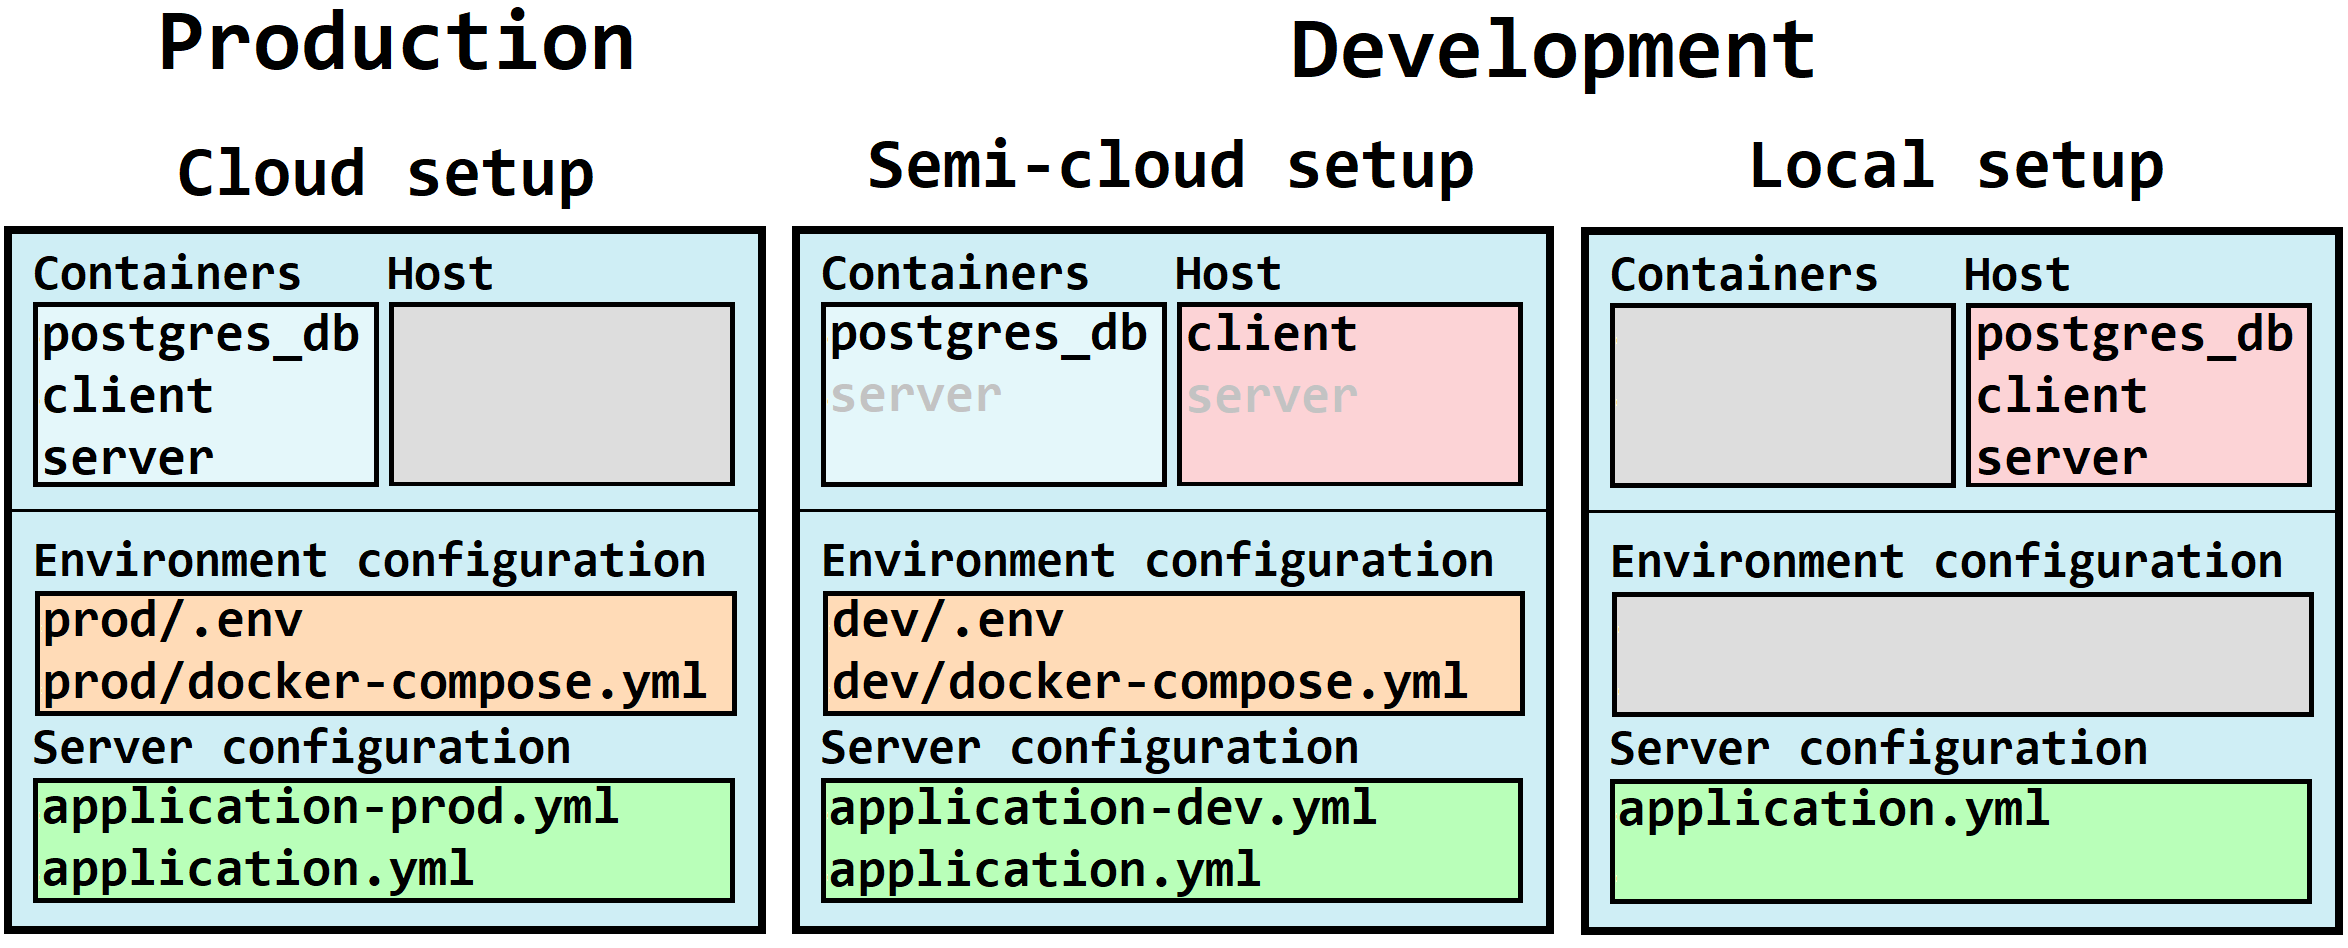
\includegraphics[width=\linewidth]{img/environments.png}
  \caption{Supported environments}
  \label{fig:2}
\end{figure}



\begin{figure}
\centering

\includegraphics[width=10cm]{logo_eng.jpg}
\caption{Figure caption (below the figure).}
\label{fig:2}
\end{figure}


\chapter{Internal specification}

\begin{itemize}
\item concept of the system
\item system architecture
\item description of data structures (and data bases)
\item components, modules, libraries, resume of important classes (if used)
\item resume of important algorithms (if used)
\item details of implementation of selected parts
\item applied design patterns
\item UML diagrams
\end{itemize}


Use special environment for inline code, eg \lstinline|descriptor| or \lstinline|descriptor_gaussian|. 
Longer parts of code put in the figure environment, eg. code in Fig. \ref{fig:pseudokod}. Very long listings–move to an appendix.

\begin{figure}
\centering
\begin{lstlisting}
class descriptor_gaussian : virtual public descriptor
{
   protected:
      /** core of the gaussian fuzzy set */
      double _mean;
      /** fuzzyfication of the gaussian fuzzy set */
      double _stddev;
      
   public:
      /** @param mean core of the set
          @param stddev standard deviation */
      descriptor_gaussian (double mean, double stddev);
      descriptor_gaussian (const descriptor_gaussian & w);
      virtual ~descriptor_gaussian();
      virtual descriptor * clone () const;
      
      /** The method elaborates membership to the gaussian fuzzy set. */
      virtual double getMembership (double x) const;
     
};
\end{lstlisting}
\caption{The \lstinline|descriptor_gaussian| class.}
\label{fig:pseudokod}
\end{figure}


\chapter{Verification and validation}
\begin{itemize}
\item testing paradigm (eg V model)
\item test cases, testing scope (full / partial)
\item detected and fixed bugs
\item results of experiments (optional)
\end{itemize}

 
 

\chapter{Conclusions}


\begin{figure}[h]
\begin{minted}[fontsize=\footnotesize, xleftmargin=-8pt, baselinestretch=1, mathescape, linenos, numbersep=4pt, frame=lines, breaklines=true, framesep=1mm]{java}
public class ColumnShuffleFacade extends AnonymisationFacade {

  AnonymisationService<ColumnShuffle> anonymisationService = new ColumnShuffleService();

  @Override
  List<Pair<String, String>> getAnonymisedRows(ColumnOperations oper, List<Pair<String, String>> rows) {
    ColumnShuffle columnShuffle = oper.getColumnShuffle();
    if (columnShuffle == null) {
      return null;
    }
    return anonymisationService.anonymise(rows, columnShuffle);
  }

  @Override
  protected AnonymisationService<ColumnShuffle> getAnonymisationService() {
    return anonymisationService;
  }
}
\end{minted}
\caption{Java code gets easily verbose.}
\label{fig:lalrpopExemplaryRule}
\end{figure}
\begin{itemize}
\item achieved results with regard to objectives of the thesis and requirements
\item path of further development (eg functional extension …)
\item encountered difficulties and problems
\end{itemize}

 
\begin{table}
\centering
\caption{A caption of a table is \textbf{above} it.}
\label{id:tab:wyniki}
\begin{tabular}{rrrrrrrr}
\toprule
	         &                                     \multicolumn{7}{c}{method}                                      \\
	         \cmidrule{2-8}
	         &         &         &        \multicolumn{3}{c}{alg. 3}        & \multicolumn{2}{c}{alg. 4, $\gamma = 2$} \\
	         \cmidrule(r){4-6}\cmidrule(r){7-8}
	$\zeta$ &     alg. 1 &   alg. 2 & $\alpha= 1.5$ & $\alpha= 2$ & $\alpha= 3$ &   $\beta = 0.1$  &   $\beta = -0.1$ \\
\midrule
	       0 &  8.3250 & 1.45305 &       7.5791 &    14.8517 &    20.0028 & 1.16396 &                       1.1365 \\
	       5 &  0.6111 & 2.27126 &       6.9952 &    13.8560 &    18.6064 & 1.18659 &                       1.1630 \\
	      10 & 11.6126 & 2.69218 &       6.2520 &    12.5202 &    16.8278 & 1.23180 &                       1.2045 \\
	      15 &  0.5665 & 2.95046 &       5.7753 &    11.4588 &    15.4837 & 1.25131 &                       1.2614 \\
	      20 & 15.8728 & 3.07225 &       5.3071 &    10.3935 &    13.8738 & 1.25307 &                       1.2217 \\
	      25 &  0.9791 & 3.19034 &       5.4575 &     9.9533 &    13.0721 & 1.27104 &                       1.2640 \\
	      30 &  2.0228 & 3.27474 &       5.7461 &     9.7164 &    12.2637 & 1.33404 &                       1.3209 \\
	      35 & 13.4210 & 3.36086 &       6.6735 &    10.0442 &    12.0270 & 1.35385 &                       1.3059 \\
	      40 & 13.2226 & 3.36420 &       7.7248 &    10.4495 &    12.0379 & 1.34919 &                       1.2768 \\
	      45 & 12.8445 & 3.47436 &       8.5539 &    10.8552 &    12.2773 & 1.42303 &                       1.4362 \\
	      50 & 12.9245 & 3.58228 &       9.2702 &    11.2183 &    12.3990 & 1.40922 &                       1.3724 \\
\bottomrule
\end{tabular}
\end{table}  

 

 


%%%%%%%%%%%%%%%%%%%%%%%%%%%%%%%%%%%%%%%%%%
\backmatter
\pagenumbering{Roman}
\stepcounter{PagesWithoutNumbers}
\setcounter{page}{\value{PagesWithoutNumbers}}

\pagestyle{onlyPageNumbers}

%%%%%%%%%%% bibliography %%%%%%%%%%%%
%\bibliographystyle{plplain} % bibtex
%\bibliography{bibliography} % bibtex
\printbibliography           % biblatex 
\addcontentsline{toc}{chapter}{Bibliography}

%%%%%%%%%  appendices %%%%%%%%%%%%%%%%%%% 

\begin{appendices} 


 

\chapter*{Index of abbreviations and symbols}
\addcontentsline{toc}{chapter}{Index of abbreviations and symbols}

\begin{itemize}
\item[DNA] deoxyribonucleic acid
\item[MVC] model--view--controller 
\item[$N$] cardinality of data set
\item[$\mu$] membership function of a fuzzy set
\item[$\mathbb{E}$] set of edges of a graph
\item[$\mathcal{L}$] Laplace transformation
\end{itemize}


\chapter*{Listings}
\addcontentsline{toc}{chapter}{Listings}

(Put long listings in the appendix.)

\begin{lstlisting}
partition fcm_possibilistic::doPartition
                             (const dataset & ds)
{
   try
   {
      if (_nClusters < 1)
         throw std::string ("unknown number of clusters");
      if (_nIterations < 1 and _epsilon < 0)
         throw std::string ("You should set a maximal number of iteration or minimal difference -- epsilon.");
      if (_nIterations > 0 and _epsilon > 0)
         throw std::string ("Both number of iterations and minimal epsilon set -- you should set either number of iterations or minimal epsilon.");
   
      auto mX = ds.getMatrix();
      std::size_t nAttr = ds.getNumberOfAttributes();
      std::size_t nX    = ds.getNumberOfData();
      std::vector<std::vector<double>> mV;
      mU = std::vector<std::vector<double>> (_nClusters);
      for (auto & u : mU)
         u = std::vector<double> (nX);
      randomise(mU);
      normaliseByColumns(mU);
      calculateEtas(_nClusters, nX, ds);
      if (_nIterations > 0)
      {
         for (int iter = 0; iter < _nIterations; iter++)
         {
            mV = calculateClusterCentres(mU, mX);
            mU = modifyPartitionMatrix (mV, mX);
         }
      }
      else if (_epsilon > 0)
      {
         double frob;
         do 
         {
            mV = calculateClusterCentres(mU, mX);
            auto mUnew = modifyPartitionMatrix (mV, mX);
            
            frob = Frobenius_norm_of_difference (mU, mUnew);
            mU = mUnew;
         } while (frob > _epsilon);
      }
      mV = calculateClusterCentres(mU, mX);
      std::vector<std::vector<double>> mS = calculateClusterFuzzification(mU, mV, mX);
      
      partition part;
      for (int c = 0; c < _nClusters; c++)
      {
         cluster cl; 
         for (std::size_t a = 0; a < nAttr; a++)
         {
            descriptor_gaussian d (mV[c][a], mS[c][a]);
            cl.addDescriptor(d);
         }
         part.addCluster(cl);
      }
      return part;
   }
   catch (my_exception & ex)                                  
   {                                                       
      throw my_exception (__FILE__, __FUNCTION__, __LINE__, ex.what()); 
   }                                                          
   catch (std::exception & ex)                                 
   {                                                            
      throw my_exceptionn (__FILE__, __FUNCTION__, __LINE__, ex.what()); 
   }                                                            
   catch (std::string & ex)                                     
   {                                                            
      throw my_exception (__FILE__, __FUNCTION__, __LINE__, ex);        
   }                                                             
   catch (...)                                                   
   {                                                             
      throw my_exception (__FILE__, __FUNCTION__, __LINE__, "unknown expection");       
   }  
}
\end{lstlisting} 

\chapter*{List of additional files in~electronic submission (if applicable)}
\addcontentsline{toc}{chapter}{List of additional files in~electronic submission (if applicable)}


Additional files uploaded to the system include:
\begin{itemize}
\item source code of the application,
\item test data,
\item a video file showing how software or hardware developed for thesis is used,
\item etc.
\end{itemize}
 
\listoffigures
\addcontentsline{toc}{chapter}{List of figures}
\listoftables
\addcontentsline{toc}{chapter}{List of tables}
	

\end{appendices}


\end{document}


%% Finis coronat opus.
